\chapter{Group Theory} \thispagestyle{empty}
\label{sec.first}

In this first chapter, the principal goal is to present (briefly) the fundamental notions of group theory we will be using in this course, and to give a sketchy idea of the groups we will study in the second half of the course.

\section{Set Theory}

In this section, we briefly recall some of the basic definitions of set theory we will be using throughout this course, and we will also introduce the notation.

\begin{definition}[Set Operations]\index{set theory!subset}\index{set theory!cartesian product}\index{set theory!difference}\index{set theory!union}\index{set theory!intersection}Let $M$ and $N$ be sets. \mbox{}
\begin{enumerate}[label=\textbf{(\alph*)}]
\item The set $M$ is a subset of $N$, and we denote it by $M \subseteq N$, if and only if
\begin{equation*}a \in M \implies a \in N. \end{equation*}
\item The set $M \cup N$ is the \textit{union} of $M$ and $N$, that is,
\begin{equation*} a \in M \cup N \iff \text{$a \in M$ \textbf{or} $a \in N$}. \end{equation*}
\item The set $M \cap N$ is the \textit{intersection} of $M$ and $N$, that is,
\begin{equation*} a \in M \cap N \iff \text{$a \in M$ \textbf{and} $a \in N$}. \end{equation*}
\item The set $N \setminus M$ is the \textit{difference} between $N$ and $M$, that is,
\begin{equation*} a \in N \setminus M \iff \text{$a \in N$ \textbf{and} $a \notin M$}. \end{equation*}
\item The set $M \times N$ is the \textit{Cartesian product} of $M$ and $N$, that is,
\begin{equation*} (a, \, b) \in M \times N \iff \text{$a \in M$ \textbf{and} $b \in N$}. \end{equation*}
Furthermore, we denote by $M^{\otimes n}$ the Cartesian product $\underbracket{M \times \dots \times M}_{n}$.
\end{enumerate} \end{definition}

\begin{definition}[Mapping] \index{mapping!injective}\index{mapping!into}\index{mapping!onto}\index{mapping!surjective}\index{mapping!bijective}\index{mapping!one-to-one} Let $M$ and $N$ be sets. \mbox{}
\begin{enumerate}[label=\textbf{(\alph*)}]
\item A mapping $f : M \longrightarrow N$ is \textit{injective} (=into) if and only if $f(b) \neq f(a)$ for every $a \neq b \in M$.
\item A mapping $f : M \longrightarrow N$ is \textit{surjective} (=onto) if and only if for every $b \in N$ there exists $a \in M$ such that $f(a) = b$.
\item A mapping $f : M \longrightarrow N$ is \textit{bijective} if and only if $f$ is both injective and surjective.
\end{enumerate}
\end{definition}
\vspace{1cm}
\begin{figure}[htbp!]
        \centering
        \mbox{%
\begin{minipage}{.40\textwidth}
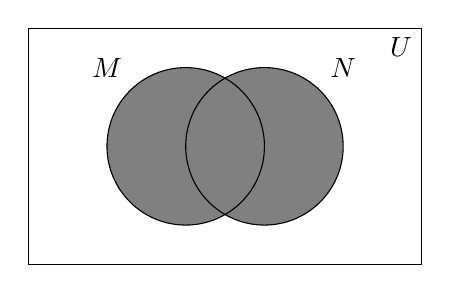
\begin{tikzpicture}
\draw (-2,-1.5) rectangle (3,1.5) node[below left]{$U$}; \fill[gray] (0,0) circle (1cm);
\fill[gray] (1,0) circle (1cm);
\draw (0,0) circle (1cm);
\draw (1,0) circle (1cm); \draw (-1,1) node {$M$}; \draw (2,1) node {$N$};
\end{tikzpicture}
          \end{minipage}%
          \qquad
          \begin{minipage}{.40\textwidth}
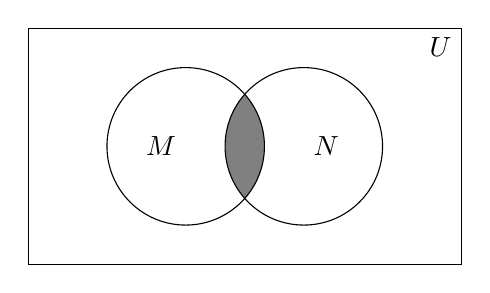
\begin{tikzpicture}
\draw (-2,-1.5) rectangle (3.5,1.5) node[below left]{$U$}; \begin{scope} % start of clip scope
\clip (0,0) circle (1cm);
\fill[gray] (1.5,0) circle (1cm);
\end{scope} % end of clip scope
\draw (0,0) circle (1cm) node[left] {$M$};
\draw (1.5,0) circle (1cm) node[right] {$N$};
\end{tikzpicture}
          \end{minipage}
    }
    \caption{Left: $M \cup N$. Right: $M \cap N$.}
\end{figure}

\begin{figure}[htbp!]
        \centering
        \mbox{%
\begin{minipage}{.40\textwidth}
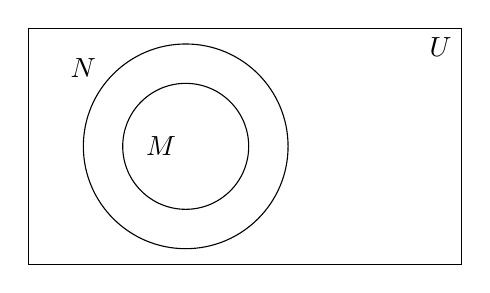
\begin{tikzpicture}
\draw (-2,-1.5) rectangle (3.5,1.5) node[below left]{$U$}; 
\draw (0,0) circle (0.8cm) node[left] {$M$};
\draw (0,0) circle (1.3cm);
\draw (-1.3, 1) node{$N$};
\end{tikzpicture}
          \end{minipage}%
          \qquad
          \begin{minipage}{.40\textwidth}
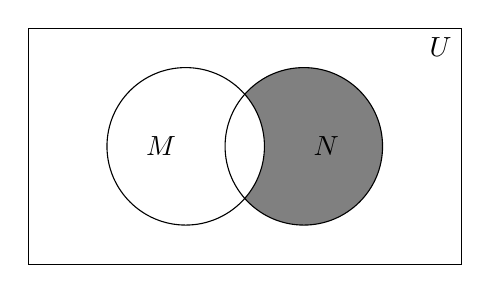
\begin{tikzpicture}
\fill[gray] (1.5, 0) circle (1cm);
\draw (-2,-1.5) rectangle (3.5,1.5) node[below left]{$U$}; \begin{scope} % start of clip scope
\clip (0,0) circle (1cm);
\fill[white] (1.5,0) circle (1cm);
\end{scope} % end of clip scope
\draw (0,0) circle (1cm) node[left] {$M$};
\draw (1.5,0) circle (1cm) node[right] {$N$};

\end{tikzpicture}
          \end{minipage}
    }
    \caption{Left: $M$ is a subset of $N$. Right: $N \setminus M$.}
\end{figure}

\vspace{1cm}

\begin{definition}[Equivalence Relation] \index{equivalence relation} Let $M$ be a set. An \textit{equivalence relation} $\sim$ is a subset of the Cartesian product $M^{\otimes 2}$ satisfying the following properties:
\begin{enumerate}[label=\textbf{(\roman*)}]
\item \textbf{\scshape Reflexive.} For every $a \in M$, it turns out that $a \sim a$.
\item \textbf{\scshape Symmetric.} For every couple $(a, \, b) \in M^{\otimes 2}$, it turns out that $a \sim b \iff b \sim a$.
\item \textbf{\scshape Transitive.} For every triple $(a, \, b, \, c) \in M^{\otimes 3}$ satisfying $a \sim b$ and $b \sim c$, it turns out that $a \sim c$.
\end{enumerate}
Moreover, given a set $M$ and an equivalence relation $\sim$, we denote by $[a]$ the \textit{equivalence class} of $a \in M$, that is,
\begin{equation*}[a] := \left\{ b \in M \: : \: b \sim a \right\}. \end{equation*} \end{definition}

\begin{example}Let $\R$ be the set of all real numbers. Then,
\begin{equation*}a \sim b \iff a - b \in \R \end{equation*}
is an equivalence relation. In fact, the reflexive property is obvious ($a - a = 0 \in \Z$ for all $a \in \R$), while the symmetric property follows from the fact that
\begin{equation*}a - b \in \Z \implies -(a-b) \in \Z \implies b - a \in \Z. \end{equation*}
The unique nontrivial property is the transitiveness, but a simple algebraic trick shows that
\begin{equation*} a - c = a \pm b - c = (a - b) + (b - c) \in Z, \end{equation*}
and this is enough to infer that $\sim$ is an equivalence relation.  \end{example}

\begin{remark}If $M$ is a set and $\sim$ an equivalence relation on $M$, then it is always possible\footnote{To prove this simple fact, it suffices to show that either $a \sim b$ or $[a]$ is disjoint from $[b]$, for all $a, \, b \in M$.} to write $M$ as the disjoint union of the equivalence classes, that is,
\caution{The set of representatives $\mathscr{R}$ is not unique!}\begin{equation*} M = \bigsqcup_{a \in \mathscr{R}} [a] \end{equation*}
where $\mathscr{R} \subset M$ denotes a maximal collection of elements $a \in M$ that are not equivalent, i.e.,
\begin{equation*} a \neq b \in \mathscr{R} \implies a \not \sim b. \end{equation*} \end{remark}

\section{Elementary Definitions and Basic Examples}

In this section, we introduce the basic definitions of group theory, and we briefly explain some of the leading examples we will be dealing with in this course.

We also present the notion of representation, which will be used in the next chapter to introduce Lie groups and Lie algebras.

\begin{definition}[Group] \index{group} A \textit{group} is a set, $\G$, together with a mapping $\cdot : \G \times \G \longrightarrow \G$, called \textit{group product}, satisfying the following properties: \mbox{}
\begin{enumerate}[label=\textbf{\arabic*)}]
\item \textbf{\scshape Closure.} For every $g_1, \, g_2 \in \G$, the product $g_1 \cdot g_2$ also belongs to $\G$.
\item \textbf{\scshape Associativity.} For every $g_1, \, g_2, \, g_3 \in \G$, it turns out that
\begin{equation*}g_1 \cdot (g_2 \cdot g_3) = (g_1 \cdot g_2) \cdot g_3. \end{equation*}
\item \textbf{\scshape Left Identity.} There exists $e \in \G$ such that $e \cdot g = g$ for every $g \in \G$.
\item \textbf{\scshape Left Inverse.} For every $g \in \G$ there exists an element, denoted by $g^{-1}$, such that
\begin{equation*}g^{-1} \cdot g = e. \end{equation*}
\end{enumerate} \end{definition}

\begin{lemma}Let $\G$ be a group, and let $g \in \G$. Then the left inverse $g^{-1}$ is also a right inverse, and the left identity $e$ is also a right identity. \end{lemma}

\begin{proof} By assumption $g^{-1} \cdot g = e$; thus the associative property implies that
\begin{equation*}g^{-1} \cdot g \cdot g^{-1} = e \cdot g^{-1} = g^{-1}, \end{equation*}
which, in turn, yields to
\begin{equation*}\underbracket{(g^{-1})^{-1} \cdot g^{-1}}_{=e} \: \cdot \: g \cdot g^{-1} =  \underbracket{(g^{-1})^{-1} \cdot g^{-1}}_{=e}.\end{equation*}
We immediately deduce that
\begin{equation*}g \cdot g^{-1} = e \cdot g \cdot g^{-1} = e,\end{equation*}
which means that $g^{-1}$ is also a right inverse for $g \in \G$. It follows from the associativity that
\begin{equation*}g^{-1} = e \cdot g^{-1} = g^{-1} \cdot g \cdot g^{-1} = g^{-1} \cdot e,\end{equation*}
which means that $e$ is also a right identity element.\end{proof}

\begin{lemma}Let $\G$ be a group. The identity element $e \in \G$ and the inverse element $g^{-1}$ are unique.\end{lemma}

\begin{proof}Suppose that $e$ and $f$ are both identity elements for a group $\G$. Then it turns out that
\begin{equation*} e = e \cdot f = f. \end{equation*}
Suppose now that $h_1, \, h_2 \in \G$ are both inverse elements for $g \in \G$. It follows from the group axioms that
\begin{equation*} h_1 = h_1 \cdot e = h_1 \cdot (g \cdot h_2) = \underbrace{(h_1 \cdot g)}_{= e} \cdot \: h_2 = h_2. \end{equation*}
\end{proof}

\begin{notation} Let $(\G, \, \cdot)$ be a group. From now on, unless there may be some ambiguity, we shall drop the product symbol $g_1 \cdot g_2$ and simply write $g_1 g_2$. \end{notation}

\begin{definition}[Abelian] \index{group!abelian} \index{group!commutative} A group $\G$ is \textit{abelian} (=commutative) if and only if
\begin{equation*}g_1 g_2 = g_2 g_1 \quad \text{for every $g_1, \, g_2 \in \G$}. \end{equation*}
\end{definition}

\begin{notation} If $\G$ is an abelian group, then the product notation ($g_1 g_2$) is usually replaced by the more comfortable additive notation ($g_1 + g_2$). Coherently, given $g \in \G$, we define
\begin{equation*} nx := \begin{cases} \underbrace{x + \dots + x}_{ \text{$n$ times} } & \text{if $n > 0$}, \\[1.5em]
- |n|x = \underbrace{- x - \dots - x}_{\text{$|n|$ times}}  & \text{if $n < 0$}, \\[1em]
 0 & \text{if $n = 0$}, \end{cases} \end{equation*}
where $0$ is the replacement for the identity element $e$ in the commutative notation.  \end{notation}

\begin{definition}[Subgroup] \index{group!subgroup} Let $(\G, \, \cdot)$ be a group. A subset $\Ha \subseteq \G$ is a \textit{subgroup} of $\G$, and we denote it by $\Ha \subgroup \G$, if $\Ha$ is a group with respect to the restriction of $\cdot$. \end{definition}

\begin{example} The set of all real numbers $\R$ is a group w.r.t. the sum $+$. The set of all integers $\Z$ is a subgroup of $\R$ since $(\Z, \, + \, \big|_{\Z})$ is a group. \end{example}

\begin{definition}[Commutator] \index{group!commutator}\index{group!center} Let $\G$ be a group. The \textit{commutator} of two elements $g_1, \, g_2 \in \G$ is defined by
\begin{equation*} [g_1, \, g_2] := g_1 g_2 g_1^{-1} g_2^{-1}. \end{equation*}
The \textit{center} of $\G$ is the set of all the elements $g \in \G$ that commute with every other element in $\G$, that is,
\begin{equation*} C(\G) := \left\{ g \in \G \: : \: \text{$[g, \, h] = e$ for every $h \in \G$} \right\}. \end{equation*}
\end{definition}

\begin{remark} The center $C(\G)$ of a group $\G$ is clearly a subgroup, and it satisfies the following properties: \mbox{}
\begin{enumerate}[label=\textbf{(\roman*)}]
\item It is an abelian subgroup of $\G$.
\item If $\G$ is an abelian group, then the commutator $[g, \, h]$ is equal to $e$ for every $g, \, h \in \G$, and the center of $\G$ coincides with $\G$.
\end{enumerate} \end{remark}

\begin{proof} \mbox{}
\begin{enumerate}[label=\textbf{(\roman*)}]
\item For every $g_1, \, g_2 \in C(\G)$ it turns out that $[g_1, \, g_2] = e$, which means that $C(\G)$ is commutative.
\item Let $g_1, \, g_2 \in \G$ be two elements. We have
\begin{equation*} [g_1, \, g_2] = g_1 \underbrace{g_2 g_1^{-1}}_{=g_1^{-1} g_2} g_2^{-1} = g_1 g_1^{-1} g_2 g_2^{-1} = e,  \end{equation*}
which means that the center coincide with the whole group $\G$. \end{enumerate} \end{proof}

\begin{definition}[Group Order] \index{group!group order} The \textit{order} of a group $\G$ is its cardinality, that is,
\begin{equation*}\mathrm{ord}(\G) := |\G|. \end{equation*}
\end{definition}

\begin{definition}[Order] \index{group!element order} Let $\G$ be a group. The \textit{order} of an element $g \in \G$ is the smallest positive integer $m \in \N$ such that\footnote{If $G$ is a group equipped with a product, we shall denote by $g^m$ the product of $m$ copies of $g$.} $g^m = e$, that is,
\begin{equation*}\mathrm{ord}(g) := \min \left\{m \in \N \: \left| \: g^m = e \right. \right\}. \end{equation*}
\end{definition}

\subsection{Main Examples in Physics}

We are now ready to briefly discuss some of the leading examples of groups, some of which will be studied more in depth later on the course.

\begin{example}[Integer Numbers] The set of all integers $\Z$ is an abelian discrete\footnote{A discrete group $\G$ is a group equipped with the discrete topology. For our purposes, it suffices to think of a group parametrized by a discrete subset of $\R$. } group with respect to the usual sum. The identity element is $0$, while the inverse element is simply given by
\begin{equation*} m^{-1} := - m \quad \text{for all $m \in \Z$}. \end{equation*}
It is important to remark that $\Z$ is \textbf{not} a group with respect to the multiplication since only $1$ and $-1$ admit a multiplicative inverse.

On the other hand, it is easy to prove that $\Q \setminus \{0\}$ is a multiplicative group with identity element $1$ and inverse $q^{-1} := \frac{1}{q}$ for $q \neq 0$. \end{example}

\begin{example}[Real Numbers] The set of all real numbers $\R$ is an abelian group with respect to the usual sum. The identity element is $0$, while the inverse element is simply given by
\begin{equation*} x^{-1} = - x \quad \text{for all $x \in \R$}. \end{equation*}
It is important to remark that $\R$ is \textbf{not} a group with respect to the usual multiplication because $0$ is not invertible.

On the other hand, one can easily prove that $\R \setminus \{0\}$ is a multiplicative group with identity element $1$ and inverse element $\frac{1}{x}$. \end{example}

\begin{example}[Symmetric Group] \index{group!symmetric group $S_3$} The \textit{symmetric group} $\mathfrak{S}_3$ consists of all the permutations of three elements. More precisely, we have
\begin{equation*} \mathfrak{S}_3 = \left\{e, \, \rho, \, \rho^2, \, \sigma, \, \rho \sigma, \, \sigma \rho \right\} \end{equation*}
where $e$ is the identity element (i.e., every element is fixed), and
\begin{equation*} \rho \: : \: \begin{aligned}1 \longmapsto 2 \\[0.5em] 2 \longmapsto 3 \\[0.5em] 3 \longmapsto 1 \end{aligned} \qquad \qquad \qquad \sigma \: : \: \begin{aligned}1 \longmapsto 2 \\[0.5em] 2 \longmapsto 1 \\[0.5em] 3 \longmapsto 3 \end{aligned} \end{equation*}
The reader may easily check that $\rho$ has order three and $\sigma$ has order two. The symmetric group $\mathfrak{S}_3$ is the first example of a non-abelian group since
\begin{equation*} (13)(2) = \rho \sigma \neq \sigma \rho = (1)(23). \end{equation*}   \end{example}

\begin{notation}The permutation $\rho$ introduced above is usually denoted by the cycle $(123)$, while $\sigma$ is denoted by $(12)(3)$ or $(12)$. In general, the permutation
\begin{equation*}(a_1 \dots a_n)(b_1 \dots b_k)(c)(d_1 \dots d_l) \end{equation*}
is given by the map that sends $a_i$ to $a_{i + 1}$ (except $a_n \mapsto a_1$), $b_i$ to $b_{i + 1}$ (except $b_k \mapsto b_1$), $c$ to itself, and $d_i$ to $d_{i + 1}$ (except $d_l \mapsto d_1$). \end{notation}

\begin{example}\index{group!symmetric group $S_n$} The \textit{symmetric group} $\mathfrak{S}_n$ consists of all the permutations of $n$ elements. \caution[c][darkgreen!50][Note]{The symmetric group $\mathfrak{S}_n$ is not abelian for all $n > 2$.}It is easy to show that $\mathfrak{S}_n$ is a discrete finite group of cardinality
\begin{equation*} |\mathfrak{S}_n| = n! \end{equation*} \end{example}

\begin{example}[Linear Transformation] \index{group!special linear group} Let $V$ be a $N$-dimensional vector space\footnote{The reader that does not recall the definition of \textit{vector space} should read \href{https://en.wikipedia.org/wiki/Vector_space}{this page} before going any further.}. The set of all $N \times N$ regular\caution{In this course we use the words "regular" and "invertible" interchangeably.} matrices with complex coefficients is a group with respect to the matrix product, and it is usually denoted by $\mathrm{GL}(N, \, \C)$. More precisely, we have
\begin{equation*}\mathrm{GL}(N, \, \C) = \left\{ A \in \mathrm{M}(N, \, \C) \: : \: \mathrm{det}(A) \neq 0 \right\}. \end{equation*}
The regular matrices with real coefficients form a subgroup, denoted by $\mathrm{GL}(N, \, \R)$, of $\mathrm{GL}(N, \, \C)$, which is given by
\begin{equation*}\mathrm{GL}(N, \, \R) = \left\{ A \in \mathrm{M}(N, \, \R) \: : \: \mathrm{det}(A) \neq 0 \right\}. \end{equation*}
In a similar fashion, the regular matrices with $\mathrm{det}(M) = 1$ also form a subgroup, called \textit{special linear group}, which is given by
\begin{equation*}\mathrm{SL}(N, \, \C) = \left\{ A \in \mathrm{GL}(N, \, \C) \: : \: \mathrm{det}(A) = 1 \right\}. \end{equation*}\end{example}

\begin{example}[Unitary Group] \index{group!unitary group} Let $V$ be a $N$-dimensional vector space. The set of all unitary complex-valued matrices \footnote{Here we denote by $U^\dag$ the transpose conjugate of a matrix $U$, that is, $U^\dag := (U^T)^\ast$.} matrices
\begin{equation*} \mathrm{U}(N, \, \C) := \left\{ U \in \mathrm{GL}(N, \, \C) \: : \: U^\dag U = U U^\dag = \mathrm{Id}_{N \times N} \right\} \end{equation*}
is a group with respect to the matrix product. Similarly,
\begin{equation*} \mathrm{SU}(N, \, \C) := \left\{ U \in \mathrm{GL}(N, \, \C) \: : \: U^\dag U = U U^\dag = \mathrm{Id}_{N \times N}, \: \mathrm{det}(U) = 1 \right\} \end{equation*}
is also a group, and it is usually called \textit{special unitary group}.\end{example}

\begin{remark} The unitary group preserves the complex scalar product
\begin{equation*}\langle z, \, w \rangle_{\C} = z^\dag \cdot w := z_1^\ast w_1^\ast + \dots + z_N^\ast w_N^\ast \quad \text{for all $z, \, w \in V$}. \end{equation*}
In fact, it is enough to notice that $U^\dag U = \mathrm{Id}_{N \times N}$, and plug it into the scalar product:
\begin{equation*} \langle z, \, w\rangle_{\C} = z^\dag \cdot w = z^\dag (U^\dag U) w = \underbrace{(z^\dag U^\dag)}_{= (Uz)^\dag} (U  w) = \langle Uz, \, Uw \rangle_{\C} \quad \text{for all $z, \, w \in V$}. \end{equation*} \end{remark}

As we will see later, this group plays a fundamental role in physics. For example, the isospin symmetry is given by the invariance of the Hamiltonian of the strong interactions under the action of the Lie group $\mathrm{SU}(2, \, \C)$.

In a similar fashion, in \hyperref[sec:apsadk]{Section \ref{sec:apsadk}} we shall prove that the Hamiltonian of the $3$-dimensional harmonic oscillator
\begin{equation*} H := \frac{\mathbf{p}^2}{2m} + \frac{m \omega^2}{2} \mathbf{r}^2 \end{equation*}
is invariant both under the action of the space rotations (i.e., the elements of $\mathrm{SO}(3, \, \R)$) and the action of the group $\mathrm{SU}(3, \, \C)$. 

\begin{example}[Orthogonal Group] \index{group!orthogonal group} Let $V$ be a $N$-dimensional vector space. The set of all the orthogonal\footnote{Here we denote by $M^T$ the transpose of  $M$.} matrices with real coefficients
\begin{equation*} \mathrm{O}(N, \, \R) := \left\{ O \in \mathrm{GL}(N, \, \R) \: : \: O^T O = O O^T = \mathrm{Id}_{N \times N} \right\} \end{equation*}
is a group with respect to the matrix product. Similarly,
\begin{equation*} \mathrm{SO}(N, \, \R) := \left\{ O \in \mathrm{GL}(N, \, \R) \: : \: O^T O = O O^T = \mathrm{Id}_{N \times N}, \: \mathrm{det}(O) = 1 \right\} \end{equation*}
is also a group, and it is called \textit{special orthogonal group}. \end{example}

\begin{remark} Notice that orthogonal matrices preserve the (real) scalar product. Indeed, we simply plug the relation $O^TO =\mathrm{Id}_{N \times N}$ into the scalar product, and we find that
\begin{equation*} \langle x, \, y\rangle = x^T \cdot y = x^T (O^T O) y = \underbrace{(x^T O^T)}_{= (Ox)^T} (O y) = \langle Ox, \, Oy \rangle \quad \text{for all $x, \, y \in V$}. \end{equation*}
More precisely, the orthogonal group $\mathrm{O}(N, \, \R)$ preserves the metric $\delta$, that is, the metric that defines the scalar product as follows:
\begin{equation*} \langle x, \, y\rangle := x_i y_j \delta^{i j}. \end{equation*}\end{remark}

\begin{example}[Symplectic Group] \index{group!symplectic group} Let $x, \, y, \, p, \, q \in \C^N$ be given vectors. The \textit{symplectic product}\index{symplectic product} between two $2N$-dimensional vectors is defined by setting
\begin{equation*} \begin{pmatrix} x_1 & \dots & x_N \: \: \vline \: \: y_1 & \dots & y_N \end{pmatrix} \cdot \begin{pmatrix} p_1 \\ \vdots \\ p_N \\ \hline q_1 \\ \vdots \\ q_N \end{pmatrix} := \sum_{i =1}^{N} \left( x_i q_i - y_i p_i \right). \end{equation*}
The group of matrices that preserve the symplectic product between $2N$-dimensional vectors is called \textit{symplectic group}, and it is usually denoted by $\mathrm{S}_p(2N, \, \C)$, or $\mathrm{S}_p(2N, \, \R)$ if the scalar field is $\R$. \end{example}

\begin{example}[Lorentz Group] \index{group!Lorentz group} The \textit{Lorentz group}, denoted by $\mathrm{O}(1, \, 3)$, is the group of all the invertible matrices $\Lambda \in \mathrm{GL}(4, \, \R)$ such that
\begin{equation}\label{eq.1.1} \Lambda^T g \Lambda = g, \end{equation}
where
\begin{equation*} g = \begin{pmatrix} 1 & 0 & 0 & 0 \\ 0 & - 1 & 0 & 0 \\ 0 & 0 & -1 & 0 \\ 0 & 0 & 0 & -1 \end{pmatrix} \end{equation*}
is the Minkwski metric with signature $(+, \, \mathbf{-})$. The transformations of the Lorentz group are thus given by
\begin{equation*}p^\mu \longmapsto \Lambda_\nu^\mu p^\nu, \end{equation*}
where $\Lambda$ is a regular matrix satisfying \eqref{eq.1.1}. \end{example}

\begin{example}[Poincaré Group] \index{group!Poincaré group} The Poincaré group, denoted by $\mathrm{P}(1, \, 3)$, is the group of all the isometries of the Minkowski space-time. More precisely, the transformations are all of the form
\begin{equation*} p^\mu \longmapsto \Lambda_\nu^\mu\,  p^\nu + b^\mu, \end{equation*}
where $\Lambda$ denotes a matrix in $\mathrm{SO}(1, \, 3)$, and $b \in \C^4$ a space-time translation. \end{example}

\begin{example}[Upper-Triangular Matrices] \index{group!triangular matrices} The set
\begin{equation*} \mathrm{UT}(2, \, \R) := \left\{ \begin{pmatrix} a & c \\ 0 & b \end{pmatrix} \: : \: a, \, b > 0, \, c \in \R \right\} \subset \mathrm{GL}(2, \, \R) \end{equation*}
is a multiplicative subgroup of the $2 \times 2$ regular matrices with real coefficients. Indeed, the identity element is given by
\begin{equation*}\mathrm{Id}_{2 \times 2} = \begin{pmatrix} 1 & 0 \\ 0 & 1 \end{pmatrix}, \end{equation*}
while the product between two elements is explicitly given by the following formula:
\begin{equation*}\begin{pmatrix} a & c \\ 0 & b \end{pmatrix} \cdot \begin{pmatrix} a^\prime & c^\prime \\ 0 & b^\prime \end{pmatrix} = \begin{pmatrix} a a^\prime & ac^\prime + c b^\prime \\ 0 & b b^\prime \end{pmatrix}. \end{equation*}
Consequently, the inverse element can be explicitly computed, and it is simply given by
\begin{equation*} \left[ \begin{pmatrix} a & c \\ 0 & b \end{pmatrix} \right]^{-1} = \begin{pmatrix} a^{-1} & -c(ba)^{-1} \\ 0 & b^{-1} \end{pmatrix}. \end{equation*} \end{example}

\begin{example}[Euclidean Group] \index{group!euclidean group} The $N$-dimensional Euclidean group, denoted by $E_N$, is the group of all transformations of the form
\begin{equation*}\R^N \ni x \longmapsto Ax + b, \end{equation*}
where $A \in O(N, \, \R)$ is an orthogonal matrix, and $b \in \R^N$ a space-translation vector. For example, if $N = 2$ every Euclidean transformation can be written in the form
\begin{equation} \label{eq.1} \begin{pmatrix} x \\ y \end{pmatrix} \longmapsto \begin{pmatrix} x^\prime \\ y^\prime \end{pmatrix} := \begin{pmatrix} \cos \theta & \sin \theta \\ - \sin \theta & \cos \theta \end{pmatrix}\begin{pmatrix} x \\ y \end{pmatrix} + \begin{pmatrix} b_1 \\ b_2 \end{pmatrix}. \end{equation}
Therefore, if we set
\begin{equation*}  R(\theta) := \begin{pmatrix} \cos \theta & \sin \theta \\ - \sin \theta & \cos \theta \end{pmatrix}, \end{equation*}
then the transformation \eqref{eq.1} can be equivalently represented in the following way
\begin{equation} \label{eq.1.2}\begin{pmatrix} x \\ y \\ 1 \end{pmatrix} \longmapsto \begin{pmatrix} x^\prime \\ y^\prime \\ 1 \end{pmatrix} = \left(\begin{array}{@{}c|c@{}}
  R(\theta) &
  \begin{matrix}
  b_1 \\
  b_2
  \end{matrix}
\\ \hline
  \begin{matrix}
  0 & 0
  \end{matrix}
  & 1
\end{array}\right) \begin{pmatrix} x \\ y \\ 1 \end{pmatrix}. \end{equation}
Denote by $E_2 \left(\mathbf{b}, \, \theta \right)$ the transformation given by \eqref{eq.1.2}. One can easily check that the product between any two elements of this form is
\begin{equation*} \begin{aligned} E_2\left( \mathbf{b}, \, \theta_1 \right) \cdot E_2 \left(  \mathbf{c}, \, \theta_2 \right) & = \left(\begin{array}{@{}c|c@{}}
  R(\theta_1) \cdot R(\theta_2) &
  R(\theta_1) \cdot \begin{pmatrix}
  c_1 \\
  c_2
  \end{pmatrix} +  \begin{pmatrix}
  b_1 \\
  b_2
  \end{pmatrix} \vspace{0.3mm}
\\ \hline
  \begin{matrix}
  0 & 0
  \end{matrix}
  & 1
\end{array}\right) =
\\[1em] & = E_2 \left(  R(\theta_1) \mathbf{c} + \mathbf{b}, \, \theta_1 + \theta_2 \right), \end{aligned} \end{equation*}
and therefore the Euclidean group $E_2$ is closed under the matrix product.

\paragraph{N.B.} The Euclidean group $E_N$ is not compact since the norm of the space-translation vector can be arbitrarily big.\end{example}

\subsection{Back to Group Theory}

To conclude this section, we now introduce more sophisticated objects (generalizing the notion of a group), and we discuss the concepts of \textit{invariant} subgroup, quotient group, and morphisms in the group category.

\begin{definition}[Ring]\index{ring}A \textit{ring} $R$ is a set with two binary operations, $+$ and $\cdot$, satisfying the following axioms: \mbox{}
\begin{enumerate}[label=\textbf{(\arabic*)}]
\item $(R, \, +)$ is an abelian/commutative group, whose identity element is denoted by $0$.
\item The multiplication $\cdot$ is associative, that is,
\begin{equation*}x_1 \cdot (x_2 \cdot x_3) = (x_1 \cdot x_2) \cdot x_3 \quad \text{for every $x_1, \, x_2, \, x_3 \in R$}. \end{equation*}
\item There exists an identity element, $1 \in R$, for the multiplication.
\item The multiplication is distributive with respect to the addition, that is,
\begin{equation*}x_1 \cdot (x_2 + x_3) = x_1 \cdot x_2 + x_1 \cdot x_3 \quad \text{and} \quad (x_2 + x_3) \cdot x_1 = x_2 \cdot x_1 + x_3 \cdot x_1. \end{equation*}
\end{enumerate}
Furthermore, a ring $R$ is said to be \textit{commutative} if and only if the multiplication $\cdot$ is commutative. \end{definition}

\begin{definition}[Field]\index{field} \index{division ring} A (commutative) ring $R$ is a (\textit{field}) \textit{division ring} if and only if every nonzero element has a multiplicative inverse, that is,
\begin{equation*} x \in R \setminus \{0\} \implies \exists \, x^{-1} \in R \: : \: x \cdot x^{-1} = x^{-1} \cdot x = 1. \end{equation*}   \end{definition}

We are finally ready to introduce the most essential definitions in group theory (i.e., quotient group, invariant subgroup, homomorphism, representation, etc.), but we first recall the notion of \textit{subgroup}, and we expand it a little bit further.

\begin{definition}[Subgroup] \index{group!subgroup} Let $(\G, \, \cdot)$ be a group. A subset $\Ha \subset \G$ is a \textit{subgroup} if $\Ha$ is a group with the restriction of $\cdot$ to $\Ha$. More precisely, we require that: \mbox{}
\begin{enumerate}[label=\textbf{\arabic*)}]
\item \textbf{\scshape Closure.} For every $h_1, \, h_2 \in \Ha$ it turns out that $h_1 \cdot h_2 \in \Ha$. 
\item \textbf{\scshape Associativity.} For every $h_1, \, h_2, \, h_3 \in \Ha$ it turns out that
\begin{equation*}h_1 \cdot (h_2 \cdot h_3) = (h_1 \cdot h_2) \cdot h_3. \end{equation*}
\item \textbf{\scshape Identity.} The identity element $e \in \G$ is also the identity element of $\Ha$.
\item \textbf{\scshape Inverse.} For every $h \in \Ha$ the inverse element $h^{-1} \in \G$ also belongs to $\Ha$.
\end{enumerate}
The singlet $\{e\}$ and the whole group $\G$ are called \textit{trivial subgroups}\index{group!trivial subgroup}. \end{definition}

\begin{definition}[Normal Subgroup] \index{group!normal subgroup}\index{group!invariant subgroup} Let $(\G, \, \cdot)$ be a group. A subgroup $\Na \subset \G$ is \textit{normal} (or \emph{invariant}), and we denote it by $\Na \trianglelefteq \G$, if and only if for every $g \in \G$ it turns out that
\begin{equation*}g h g^{-1} \in \Na \quad \text{for every $h \in \Na$}. \end{equation*} \end{definition}

\begin{exercise} Prove that a subgroup $\Na$ of a group $\G$ is normal if and only if
\begin{equation*}g \Na g^{-1} \subseteq \Na \quad \text{for every $g \in \G$}. \end{equation*}\end{exercise}

Let $\Na \trianglelefteq \G$ be a normal subgroup. We introduce an equivalence relation on the elements of $\G$ in the following way:
\begin{equation*}g \sim_{\Na} h \iff gh^{-1} \in \Na \iff g \in h \cdot \Na. \end{equation*}
Let $\mathscr{R} \subset \G$ be a set of representatives. The set of the equivalence classes $[g] := g \cdot \Na$ is called \textit{quotient group}, and it is denoted by
\begin{equation*} \faktor{\G}{\Na} := \left\{ [g] \: : \: g \in \mathscr{R} \right\}. \end{equation*}
The reader should check that $\faktor{\G}{\Na}$ is actually a group with the following operation:
\caution{If $\Ha \subgroup \G$ is not normal, then the quotient is well defined, even thought is not a group. It is a "set with a left group action" instead.}\begin{equation*} [g] \cdot [h] := [gh], \end{equation*}
which is well-defined as a consequence of the fact that $\Na$ is a \underline{normal} subgroup!

\begin{definition}[Simple Group] \index{group!simple group} A group $\G$ is said to be \textit{simple} if the normal subgroups are the trivial ones only, that is,
\begin{equation*} \text{$\Na \trianglelefteq \G$} \implies \text{$\Na = \{e\}$ or $\Na = \G$}.\end{equation*}
\end{definition}

\begin{definition}[Semisimple Group] \index{group!semisimple group} A group $\G$ is said to be \textit{semisimple} if any normal subgroups (except for $\{e\}$) is not abelian, that is,
\begin{equation*} \text{$\Na \trianglelefteq \G$} \implies \text{$\Na$ is not abelian or $\Na = \{e\} $}.\end{equation*}
\end{definition}

\begin{definition}[Direct Product] \index{group!direct product} Let $\G$ and $\G^\prime$ be two groups. The \textit{direct product} $\G \otimes \G^\prime$ is given by the set of all couples $(g, \, g^\prime) \in \G \times \G^\prime$ together with the following operation:
\begin{equation*} (g_1, \, g_1^\prime) \cdot (g_2, \, g_2^\prime) := (g_1 g_2, \, g_1^\prime g_2^\prime). \end{equation*} \end{definition}

\begin{remark} The direct product is a group, but it can never be simple since the subgroups
\begin{equation*} \Ha := \G \times \{e^\prime\} \quad \text{and} \quad \Ha^\prime := \{e\} \times \G^\prime\end{equation*}
are both nontrivial and normal. In a similar fashion, one can easily prove that a direct product $\G \otimes \G^\prime$ is semisimple if and only if both $\G$ and $\G^\prime$ are semisimple. \end{remark}

\begin{theorem}[Direct Decomposition] Let $\G$ be a group, and let $\Ha, \, \mathcal{K} \subgroup \G$. Suppose that the following properties hold true: \mbox{}
\begin{enumerate}[label=\textbf{(\arabic*)}]
\item The subgroups $\Ha$ and $\mathcal{K}$ are normal, that is, $\Ha, \, \mathcal{K} \trianglelefteq \G$.
\item The intersection between $\Ha$ and $\mathcal{K}$ is trivial, that is, $\Ha \cap \mathcal{K} = \{e\}$.
\item Every element $g \in \G$ can be written as the product of an element $h \in \Ha$ and an element $k \in \mathcal{K}$, that is, $\G = \Ha \mathcal{K}$.
\end{enumerate}
Then $\G$ is isomorphic to the direct product $\Ha \otimes \mathcal{K}$.\end{theorem}

\begin{definition}[Homomorphism] \index{group!homomorphism} A mapping $\varphi : \G \longrightarrow \G^\prime$ between two groups is a \textit{homomorphism} (of groups) if it is compatible with the group structure, that is,
\begin{equation*} \varphi( g_1 \cdot g_2 ) = \varphi(g_1) \cdot \varphi(g_2) \quad \text{for all $g_1, \, g_2 \in \G$}. \end{equation*}  \end{definition}

\begin{lemma}If $\varphi : \G \longrightarrow \G^\prime$ is a homomorphism of groups, then
\begin{equation*} \varphi(e) = e^\prime \quad \text{and} \quad \left( \varphi(g) \right)^{-1} = \varphi(g^{-1}) \end{equation*}
for every $g \in \G$. \end{lemma}

\begin{proof} The first property follows immediately by noticing that
\begin{equation} \label{eq.1.3} \varphi(e) = \varphi(e \cdot e) = \varphi(e) \cdot \varphi(e) \implies \varphi(e) = e^\prime. \end{equation}
Fix $g \in \G$. By \eqref{eq.1.3} it turns out that
\begin{equation*} \begin{aligned} & \varphi(g^{-1}) \cdot \varphi(g) = \varphi(g^{-1} \cdot g) = \varphi(e) = e^\prime, \\[0.8em]  & \varphi(g) \cdot \varphi(g^{-1}) = \varphi(g \cdot g^{-1}) = \varphi(e) = e^\prime, \end{aligned} \end{equation*}
which means that $\varphi(g^{-1})$ is the inverse of $\varphi(g)$. \end{proof}

\begin{definition}[Isomorphism] \index{group!isomorphism} A group homomorphism $\varphi : \G \longrightarrow \G^\prime$ is an \textit{isomorphism} if $\varphi$ is one-to-one (i.e., injective and surjective).\end{definition}

If $\G$ and $\G^\prime$ are two groups, we will say that $\G$ is isomorphic to $\G^\prime$ (and vice versa) if and only if there exists a group isomorphism $\varphi : \G \longrightarrow \G^\prime$, and we will write $\G \cong \G^\prime$.

\begin{definition}[Automorphism] \index{group!automorphism} A group homomorphism $\varphi : \G \longrightarrow \G$ is an \textit{automorphism} if $\varphi$ is a group isomorphism.\end{definition}

\begin{remark}Let $\G$ be a group. The set of all the automorphisms of $\G$ is a group with the composition, and it is usually denoted by $(\mathrm{Aut}(\G), \, \circ)$. Indeed,
\begin{equation*}\begin{aligned} & \varphi_2 \circ \varphi_1 \in \mathrm{Aut}(\G), \\[0.8em]
& \varphi_1 \circ \mathrm{id}_\G = \mathrm{id}_\G \circ \varphi_1 = \varphi_1, \\[0.8em]
\end{aligned}\end{equation*}
for every $\varphi_1, \, \varphi_2 \in \mathrm{Aut}(\G)$, and the inverse element is given by the usual inverse $\varphi^{-1}$, which exists as the mappings are all one-to-one.\end{remark}

\begin{definition}[Conjugation] \index{group!conjugate}\index{group!conjugation} Let $\G$ be a group. For every $g \in \G$ the \textit{conjugation} with respect to $g$ is defined by setting
\begin{equation*}\varphi_g : \G \ni h \longmapsto g h g^{-1} \in \G. \end{equation*}\end{definition}

The reader may easily prove that the conjugations $\varphi_g$ form a subgroup of $\mathrm{Aut}(\G)$, which is usually called the group of the \textit{inner automorphisms} and denoted by $\mathrm{Inn}(\G)$.  

\begin{definition}[Kernel] \index{group!homomorphism!kernel} Let $\varphi : \G \longrightarrow \G^\prime$ be a group homomorphism. The kernel of $\varphi$ is the set of all the $g \in \G$ with image (via $\varphi$) the identity element $e^\prime$, that is,
\begin{equation*}\mathrm{ker}(\varphi) := \left\{ g \in \G \: : \: \varphi(g) = e^\prime \right\} = \varphi^{-1}(e^\prime). \end{equation*} \end{definition}

\begin{lemma}The kernel of a group homomorphism $\varphi : \G \longrightarrow \G^\prime$ is a normal subgroup. \end{lemma}

\begin{proof} For every $h \in \mathrm{ker}(\varphi)$ and $g \in \G$ it turns out that
\begin{equation*}\varphi ( ghg^{-1} ) = \varphi(g) \underbrace{\varphi(h)}_{= e^\prime} \varphi(g)^{-1} = \varphi(g) \varphi(g)^{-1} = e^\prime, \end{equation*}
which means that
\begin{equation*}g \cdot \mathrm{ker}(\varphi) \cdot g^{-1} \subseteq \mathrm{ker}(\varphi) \quad \text{for every $g \in \G$}.  \end{equation*}\end{proof}

\begin{lemma}Let $\varphi : \G \longrightarrow \G^\prime$ be a group homomorphism, and let $\K$ be its kernel. Then the induced group homomorphism
\begin{equation*} \widetilde{\varphi} : \faktor{\G}{\K} \longrightarrow \G^\prime \end{equation*}
is injective. \end{lemma}

\begin{proof}The induced homomorphism is defined as follows:
\begin{equation*} \widetilde{\varphi}([g]) := \varphi(h) \quad \text{for every $h \in [g]$}. \end{equation*}
Therefore, if $[g_1], \, [g_2] \in \faktor{\G}{\K}$ have the same image via $\widetilde{\varphi}$, then
\begin{equation*} \varphi(g_1) = \varphi(g_2) \implies \varphi(g_1 g_2^{-1}) = e^\prime, \end{equation*}
which means that $g_1 g_2^{-1} \in \K$. In particular,
\begin{equation*}g_1 \in g_2 \cdot \K \implies [g_1] = [g_2] \implies \text{$\widetilde{\varphi}$ is injective}.\end{equation*}
\end{proof}

\begin{definition}[Representation] \index{representation} A \textit{representation} of a group $\G$ on a $N$-dimensional vector space $V$ over a field $\mathbb{K}$ is a group homomorphism
\begin{equation*} \rho : \G \longrightarrow \mathrm{GL}(N, \, \mathbb{K}; \; V), \end{equation*}
that is, a mapping $\rho$ such that $\rho(g_1 g_2) = \rho(g_1) \cdot \rho(g_2)$ for every $g_1, \, g_2 \in \G$, where $\cdot$ denotes the matrices product. \end{definition}

In particular, the identity element $e \in \G$ is represented by the identity matrix $\mathrm{Id}_{N \times N}$, while the inverse element $g^{-1}$ is represented by the inverse matrix $\rho(g)^{-1}$.

Moreover, every group $\G$ admits a trivial $1$-dimensional representation\index{trivial representation}, which is defined in the following way:
\begin{equation*}\rho(g) := (1)\quad\text{for all $g \in \G$}. \end{equation*}

\begin{definition}[Similarity] \index{representation!equivalence} Let $\G$ be a group, and let $\{\rho, \, V\}$ and $\{\widetilde{\rho}, \, \widetilde{V} \}$ be two $N$-dimensional representations of $\G$. We say that they are \textit{similar} (or, equivalent) if and only if there exists a regular (=invertible) matrix $S$ such that
\begin{equation*} \widetilde{\rho}(g) = S \rho(g) S^{-1} \quad \text{for every $g \in \G$}. \end{equation*}
\end{definition}

\begin{definition}[Unitary Representation] \index{representation!unitary} A $N$-dimensional representation $\{ \rho, \, V \}$ of a group $\G$ is \textit{unitary} if and only if $\rho(g) \in \mathrm{U}(N, \, \C)$ for every $g \in \G$. \end{definition}

\begin{definition}[Compact Group] \index{group!compact} A compact group $\G$ is a topological group whose topology is compact\footnote{For our purposes, it suffices to define a compact group as a group which depends on a finite number of real parameters and these parametters are limited.}.\end{definition}

\section{Finite Groups}

In this brief section, we introduce some basic examples of \textit{finite} group. More precisely, we shall ultimately characterize the finite groups of order $n = 2, \, 3$ and $4$, and introduce the symmetric and dihedral groups.

{\centering \subsection*{Order $2$.} }

There exists a unique group of order $2$, and it is the cyclic group $\mathcal{C}_2 = \{e, \, a\}$. The product $\cdot$ is uniquely determined by the group axioms, and we have that
\begin{equation*}a \cdot a = e \implies a = a^{-1}. \end{equation*}
In particular, the group $\mathcal{C}_2$ admits a $1$-dimensional representation which is given by
\begin{equation*}  \rho(e) = 1 \quad \text{and} \quad \rho(a) = -1. \end{equation*}
Moreover, the cyclic group $\mathcal{C}_2$ is isomorphic to the group $\Z_2 = \{ 0, \, 1 \}$ equipped with the sum modulo $2$, that is,
\begin{equation*} 1 + 1 \equiv_{2} = 0 \implies 1 \equiv_{2} - 1. \end{equation*}

{\centering \subsection*{Order $3$.} }

There exists a unique group of order $3$, and it is the cyclic group $\mathcal{C}_3 = \{e, \, a, \, b\}$. The product $\cdot$ is uniquely determined by the group axioms, and we have that
\begin{equation*} \begin{aligned} & a \cdot a = b, \\[0.6em] & a \cdot b = e,  \\[0.6em] & b \cdot b = a. \end{aligned}\end{equation*}
In particular, the group $\mathcal{C}_3$ admits a $1$-dimensional representation which is given by the complex solutions of the equation $z^3 = 1$, that is,
\begin{equation*}  \rho(e) = 1 \quad \text{and} \quad \rho(a) = \mathrm{e}^{\frac{2 \imath \pi}{3}} \quad \text{and} \quad \rho(b) = \mathrm{e}^{\frac{4 \imath \pi}{3}}. \end{equation*}
Moreover, the cyclic group $\mathcal{C}_3$ is isomorphic to the group $\Z_3 = \{ 0, \, 1, \, 2 \}$ equipped with the sum modulo $3$.

\vspace{6mm}
\begin{figure}[!htbp]
        \centering
        \mbox{%
\begin{minipage}{.45\textwidth}
\begin{tikzpicture}
\draw (0,0) circle (3cm);
[anchor=mid west,
  mark size=+2pt, mark color=red,  ball color=green]
  \foreach \plm[count=\cnt] in {ball}
    \draw[mark options={fill=red}]
      plot[mark=\plm] coordinates {(3, 0) (-3, 0)};
\end{tikzpicture}
          \end{minipage}%
          \qquad
          \begin{minipage}{.45\textwidth}
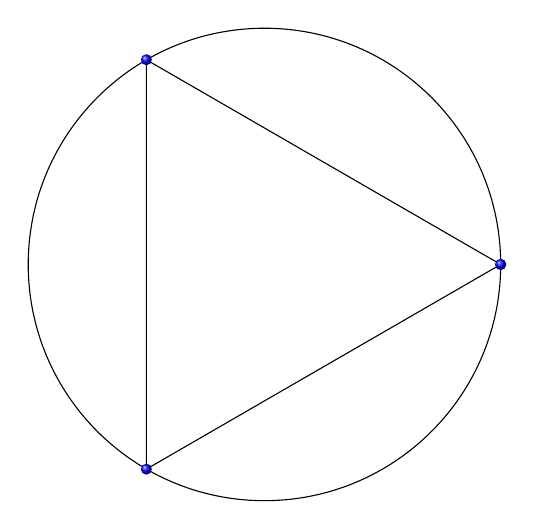
\begin{tikzpicture}
\draw (0,0) circle (3cm);
[anchor=mid west,
  mark size=+2pt, mark color=red,  ball color=green]
  \foreach \plm[count=\cnt] in {ball}
    \draw[mark options={fill=red}]
      plot[mark=\plm] coordinates {(3, 0) (-1.5, 2.6) (-1.5, -2.6) (3, 0)};
\end{tikzpicture}
          \end{minipage}
    }
    \caption{\textbf{Left:} $1$-dimensional representation of $\mathcal{C}_2$. \textbf{Right:} $1$-dimensional representation of $\mathcal{C}_3$.}
\end{figure}

{\centering \subsection*{Order $n$.} }

The notion of cyclic group can be easily generalized for every natural number $n \in \N$. Indeed, the $n$th cyclic group is given by
\begin{equation*} \mathcal{C}_n = \{a_0 := e, \, a_1, \, \dots, \, a_{n - 1} \} \end{equation*}
and the product $\cdot$ is uniquely determined by the group axioms, that is,
\begin{equation*} a_i \cdot a_j = \begin{cases} a_{i + j} & \text{if $i + j < n$}, \\[0.8em] a_{i + j - n} & \text{if $i + j \geq n$}. \end{cases} \end{equation*}
In particular, the cyclic group $\mathcal{C}_n$ is isomorphic to
\begin{equation*} \mathcal{C}_n = \{e, \, a, \, a^2, \, \dots, \, a^{n-1} \: : \: a^n = e \}, \end{equation*}
as the reader may easily check that the map
\begin{equation*} \varphi(a_i) := a^i \quad \text{for every $i = 0, \, \dots, \, n - 1$} \end{equation*}
is an isomorphism. Moreover, the group $\mathcal{C}_n$ admits a $1$-dimensional representation which is given by the complex solutions of the equation $z^n = 1$, that is,
\begin{equation*}  \rho(a_j) = \mathrm{e}^{ \imath \frac{2\pi j}{n} } \quad \text{for every $j \in \{0, \, \dots, \, n - 1\}$}. \end{equation*}
Furthermore, the cyclic group $\mathcal{C}_n$ is isomorphic, for every $n \in \N$, to the group $\Z_n = \{ 0, \, 1, \, \dots, \, n - 1 \}$ equipped with the sum modulo $n$.

\begin{figure}[!htbp]
        \centering
        \mbox{%
\begin{minipage}{.45\textwidth}
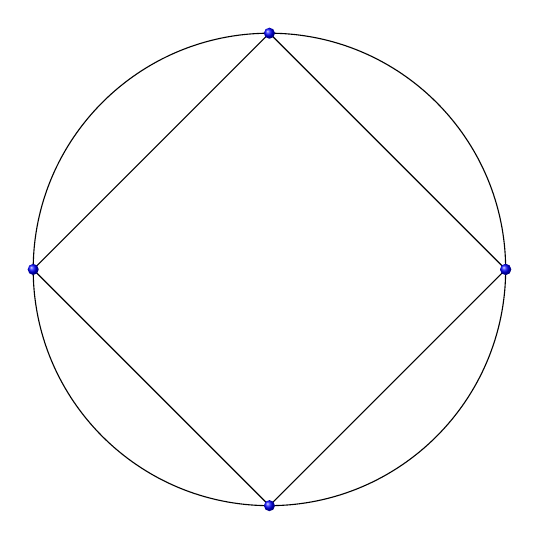
\begin{tikzpicture}
\draw (0,0) circle (3cm);
[anchor=mid west,
  mark size=+2pt, mark color=red,  ball color=green]
  \foreach \plm[count=\cnt] in {ball}
    \draw[mark options={fill=red}]
      plot[mark=\plm] coordinates {(3, 0) (0, 3) (-3, 0) (0, -3) (3, 0)};
\end{tikzpicture}
          \end{minipage}%
          \qquad
          \begin{minipage}{.45\textwidth}
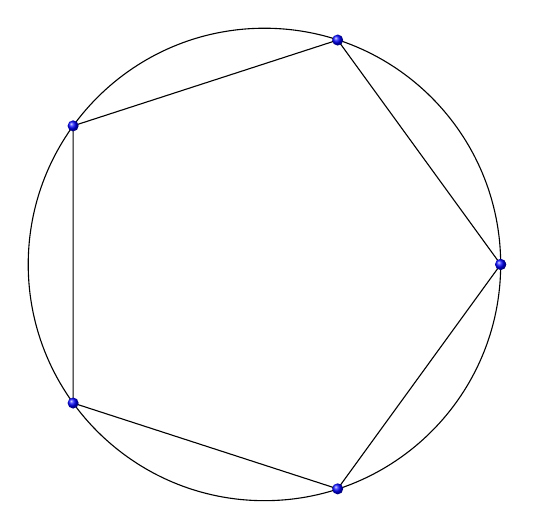
\begin{tikzpicture}
\draw (0,0) circle (3cm);
[anchor=mid west,
  mark size=+2pt, mark color=red,  ball color=green]
  \foreach \plm[count=\cnt] in {ball}
    \draw[mark options={fill=red}]
      plot[mark=\plm] coordinates {(3, 0) (0.93, 2.85)  (-2.43, 1.76) (-2.43, - 1.76) (0.93, -2.85) (3, 0)};
\end{tikzpicture}
          \end{minipage}
    }
    \caption{\textbf{Left:} $1$-dimensional representation of $\mathcal{C}_4$. \textbf{Right:} $1$-dimensional representation of $\mathcal{C}_5$.}
\end{figure}

{\centering \subsection*{Order $4$.} }

The cyclic group $\mathcal{C}_4$ is the unique abelian group of order $4$, but there is also a non cyclic group, called \textit{dihedral group} and denoted by $\mathcal{D}_2$.

The \textbf{dihedral group} of order $2$ is given by the symmetries of a rectangle, which means that there is the identity element $e$, a rotation $R_{\pi}$ of angle $\pi$, the reflection $S_x$ with respect to the $x$-axis, and the reflection $S_y$ with respect to the $y$-axis.

The group $\mathcal{D}_2$ is isomorphic to the Klein group $\mathcal{K}_4$, but it is not isomorphic to the cyclic group of order $4$. To prove this assertion, it suffices to notice that
\begin{equation*} \begin{aligned}& \text{$\mathcal{C}_4$ is cyclic} \implies \mathcal{C}_4 = \{e, \, a, \, a^2, \, a^3 \}, \\[1em] & \text{$\mathcal{D}_2 = \{e, \, R_\pi, \, S_x, \, S_y \}$ and $R_\pi^2 = S_x^2 = S_y^2 = e$} \implies \text{$\mathcal{D}_2$ is not cyclic}. \end{aligned} \end{equation*}

\begin{figure}[!htbp]
        \centering
        \mbox{%
\begin{minipage}{.50\textwidth}
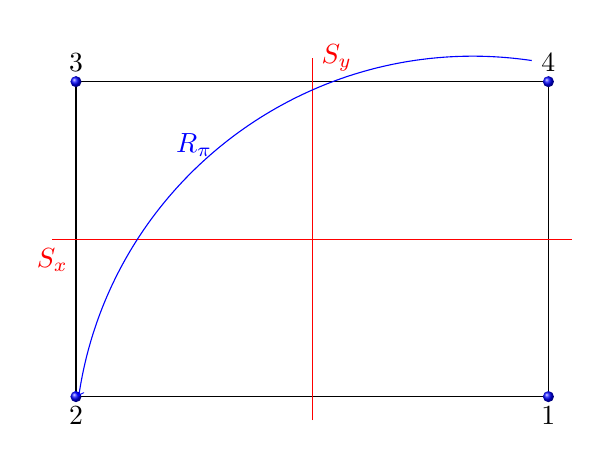
\begin{tikzpicture}
\draw (-3,-2) rectangle (3,2); 
\draw[-,ultra thin, red] (-3.3,0)--(3.3,0) node[pos = 0, below]{$S_x$};
\draw[-,ultra thin, red] (0, -2.3)--(0,2.3) node[right]{$S_y$};
[anchor=mid west,
  mark size=+2pt, mark color=red,  ball color=green]
  \foreach \plm[count=\cnt] in {ball}
    \draw[mark options={fill=red}]
      plot[mark=\plm] coordinates {(3, -2)} node[below]{1};
      [anchor=mid west,
  mark size=+2pt, mark color=red,  ball color=green]
  \foreach \plm[count=\cnt] in {ball}
    \draw[mark options={fill=red}]
      plot[mark=\plm] coordinates {(-3, -2)} node[below] (2) {2};
      [anchor=mid west,
  mark size=+2pt, mark color=red,  ball color=green]
  \foreach \plm[count=\cnt] in {ball}
    \draw[mark options={fill=red}]
      plot[mark=\plm] coordinates {(3, 2)} node[above] (4) {4};
      [anchor=mid west,
  mark size=+2pt, mark color=red,  ball color=green]
  \foreach \plm[count=\cnt] in {ball}
    \draw[mark options={fill=red}]
      plot[mark=\plm] coordinates {(-3, 2)} node[above]{3};
\draw[->, blue] (4) to [bend right=45] (2);
\node[blue] (A) at (-1.5,1.2) {$R_\pi$};
\end{tikzpicture}
          \end{minipage}%
          \qquad
          \begin{minipage}{.50\textwidth}
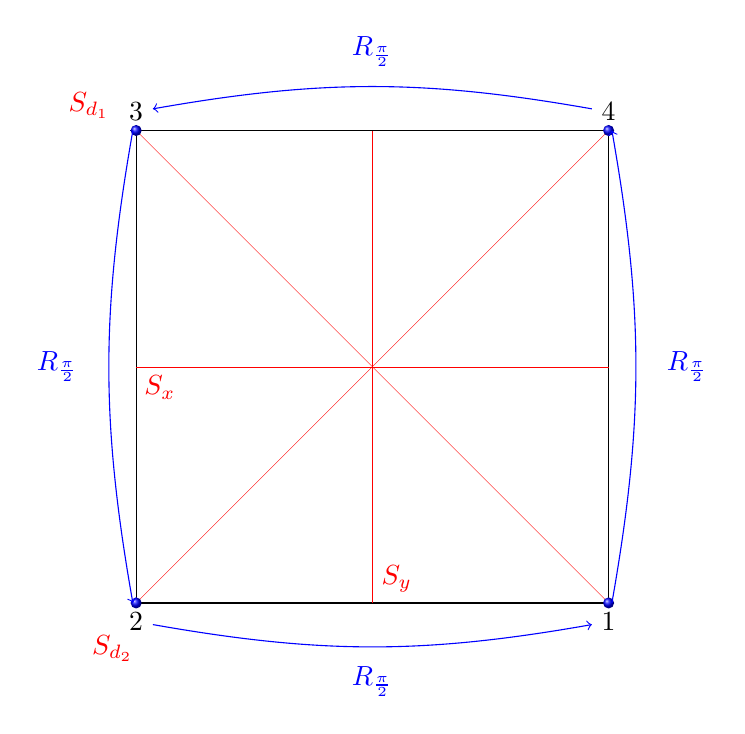
\begin{tikzpicture}
\draw (-3,-3) rectangle (3,3); 
\draw[-,ultra thin, red] (-3,0)--(3,0) node[pos = 0.05, below]{$S_x$};
\draw[-,ultra thin, red] (0, -3)--(0,3) node[right, pos = 0.05]{$S_y$};
\draw[-,ultra thin, red] (-3,3)--(3,-3) node[pos = -0.10, below]{$S_{d_1}$};
\draw[-,ultra thin, red] (-3,-3)--(3, 3) node[pos = -0.05, below]{$S_{d_2}$};
[anchor=mid west,
  mark size=+2pt, mark color=red,  ball color=green]
  \foreach \plm[count=\cnt] in {ball}
    \draw[mark options={fill=red}]
      plot[mark=\plm] coordinates {(3, -3)} node[below](1){1};
      [anchor=mid west,
  mark size=+2pt, mark color=red,  ball color=green]
  \foreach \plm[count=\cnt] in {ball}
    \draw[mark options={fill=red}]
      plot[mark=\plm] coordinates {(-3, -3)} node[below] (2) {2};
      [anchor=mid west,
  mark size=+2pt, mark color=red,  ball color=green]
  \foreach \plm[count=\cnt] in {ball}
    \draw[mark options={fill=red}]
      plot[mark=\plm] coordinates {(3, 3)} node[above] (4) {4};
      [anchor=mid west,
  mark size=+2pt, mark color=red,  ball color=green]
  \foreach \plm[count=\cnt] in {ball}
    \draw[mark options={fill=red}]
      plot[mark=\plm] coordinates {(-3, 3)} node[above](3) {3};
\draw[->, blue] (4) to [bend right=10] (3);
\draw[->, blue] (3) to [bend right=10] (2);
\draw[->, blue] (2) to [bend right=10] (1);
\draw[->, blue] (1) to [bend right=10] (4);
\node[blue] (A) at (0, 4) {$R_{\frac{\pi}{2}}$};
\node[blue] (B) at (4, 0) {$R_{\frac{\pi}{2}}$};
\node[blue] (C) at (-4, 0) {$R_{\frac{\pi}{2}}$};
\node[blue] (D) at (0, -4) {$R_{\frac{\pi}{2}}$};
\end{tikzpicture}
          \end{minipage}
    }
    \caption{\textbf{Left:} Dihedral group $\mathcal{D}_2$. \textbf{Right:} Dihedral group $\mathcal{D}_4$.}
\end{figure}

{\centering \subsection*{Dihedral Group $2n$.} }

 The $n$th dihedral group $\mathcal{D}_n$ has order $2n$ and consists of all the regular isometries of the plane that preserve the regular polygons with $n$ edges. More precisely, we have
\begin{equation*} \mathcal{D}_n = \{e, \, \rho, \, \dots, \, \rho^{n - 1}, \, S_1, \, \dots, \, S_n \}, \end{equation*}
where $\rho$ is the rotation of angle $\frac{2 \pi}{n}$, in such a way that $\rho^j$ is the rotation of angle $\frac{2 \pi}{n} j$, and $S_i$ is the reflection with respect to the $i$th axis of symmetry. The reader may check by herself that
\begin{equation*} \mathcal{D}_n = \{e, \, \rho, \, \dots, \, \rho^{n-1}, \, S, \, S \rho, \, \dots, \, S \rho^{n - 1} \}, \end{equation*}
for any reflection $S := S_i$. Moreover, a straightforward computation proves that
\begin{equation} \label{eq.7.1} \rho^k S = S \rho^{n - k} \quad \text{for every $k \in \{0, \, \dots, \, n - 1\}$}. \end{equation}
The $n$th dihedral group $\mathcal{D}_n$ is completely characterized by these properties: It is generated by a rotation $\rho$ of order $n$ and a symmetry $S$ of order $2$ satisfying the relation \eqref{eq.7.1}.